\documentclass[12pt,a4paper]{article}
\usepackage[top=25.4mm, bottom=25.4mm, left=19.1mm, right=19.1mm]{geometry}

\usepackage[latin2]{inputenc}
\usepackage{graphicx}
\graphicspath{ {./images/} }
\usepackage{ulem}
\usepackage{amsmath}
\usepackage[document]{ragged2e}

\setlength{\parindent}{4em}
\setlength{\parskip}{1em}
\usepackage{hyperref}

\usepackage{fancyhdr}
\pagestyle{fancy}
\fancyhf{}
\fancyhead[LO]{\textbf{\small IoT and Smart Analytics}\\
\text{\small A Program by IIITH and TalentSprint}}

\usepackage{xcolor}
\usepackage{lipsum}

\rhead{\begin{picture}(0,0) \put(-250,-2){
\includegraphics[width=9cm]{EXP_08_Images/ts-iisc-logo-pr.png}} \end{picture}}
\cfoot{\thepage}


\begin{document}

\begin{center}

\textbf{\large \\EXPERIMENT 09 }\\[6pt]
\text{Analog output using RC filter and Arduino UNO}
\end{center}

\textbf{\large LEARNING OBJECTIVES:}\\[3pt]
At the end of this experiment, participants will be able to:\vspace{-6mm}\begin{enumerate}
 \setlength\itemsep{-0.3em}
\item Understand pulse width modulation \\
\item Use RC filter to output constant DC signal \\

\end{enumerate}
\textbf{\large APPARATUS REQUIRED:}\\
\vspace{-3mm}
\begin{enumerate}
 \setlength\itemsep{-0.3em}
\item Arduino Module-2pcs \\
\item Power Adapter-1pcs\\
\item Breadboard-1pcs\\
\item Capacitor-1pcs\\
\item Resistor 4.7k$\Omega$ -1pcs\\
\item Jumper wires\\

\end{enumerate}

\begin{justify}
\textbf{\large THEORY}\\[3pt]
\textbf{Pulse Width Modulation: } PWM is a digital square wave signal that oscillates according to a given frequency and duty cycle. The frequency which is expressed in Hertz (Hz) describes how often the output pulse repeats. The period is defined as the time each cycle takes and is the inverse of frequency. The duty cycle, which is mentioned as a percentage, describes the pulse's width within that frequency window.\par
\noindent The duty cycle can be adjusted to increase or decrease the signal's average "on" time. Fig.1 shows pulse trains at 10\%, 50\%, and 90\% duty.\par
\noindent \textbf{The Problem with analogWrite(): } The Arduino can read analog voltages between 0 and 5 volts using the analogRead() function. The next question that arises is there a way for the Arduino to output analog voltages as well? The answer is a bit confusing. Arduino UNO, however, does not have true analog voltage. As Arduino is so fast, it can fake it using PWM ("Pulse-Width Modulation"). The pins on the Arduino with ~ (Tilda) next to them are PWM compatible. Arduino is so fast that it can on and off a pin almost a thousand times per second. Also, PWM goes one step further by varying the amount of time the blinking pin spends HIGH vs. the time it spends LOW, i.e., the duty cycle. If it spends most of its time ON, an LED connected to the pin will appear bright. And if it spends most of its time OFF, the LED will look dim. Because the pin is blinking very much faster than our eye can detect, it creates the illusion of a "true" analog output. For an even more smooth signal, we will create and use an RC circuit that acts as a Lowpass Filter and allows only constant output. 

\begin{center} 
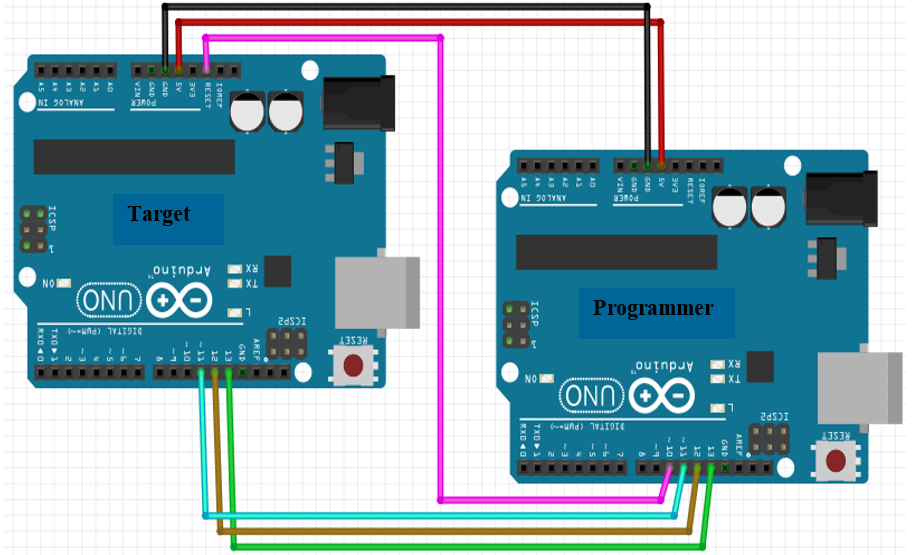
\includegraphics[scale=0.9]{EXP_09_Images/fig1.png}
\end{center}
\begin{center} {Figure 1. Pulse Width Modulation}\end{center}

\noindent The Arduino makes PWM easy to use by simply calling analogWrite(pin, duty cycle), whereas duty cycle is a value between 0 to 255, and a pin is one of the PWM pins, which are 3, 5, 6, 9, 10, or 11 on Arduino UNO. The function provides a simple interface to the hardware PWM. But it doesn't control the frequency and is fixed to 490 Hz. We can use any other digital pin to emulate the PWM functionality using digitalWrite() and delay. Note: Despite the name of the function, the output is a digital signal, a square wave. \par
\noindent \textbf{Arduino Analog Out:  }Arduino UNO has no true built-in Analog Output Channels (only PWM) so we are going to use and examine an RC Lowpass Filter that converts PWM to Voltage.

\begin{center} 
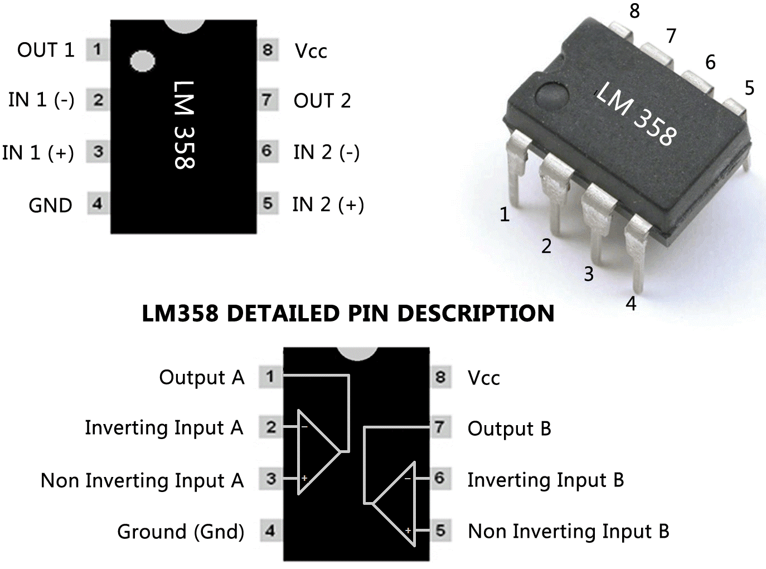
\includegraphics[scale=0.8]{EXP_09_Images/fig2.png}
\end{center}
\begin{center} {Figure 2. RC circuit }\\[21pt]\end{center}

\noindent If we examine the circuit in Fig.2, when a voltage is applied to the input of Resistor R, the capacitor C will begin charging. When it is charged, it will stop to conduct current, and the voltage at the output of this circuit will match the input. Note that the capacitors block the DC currents but pass the AC currents, you can see that any of the DC voltage input will also be output, but high-frequency AC voltages will be shorted to the ground. The lower frequency AC voltages will be filtered according to the RC time constant formed by the resistor and capacitor network. While this circuit is very simple to understand and use, choosing the appropriate values for R & C encompasses some design decisions. Like, how much ripple can we tolerate, and how fast does the filter need to respond? These two parameters are mutually exclusive. We would like to have the perfect filter that passes all frequencies below the cutoff frequency, with no voltage ripple. While no ideal filter exists, it is possible to achieve close to it by using a multiple pole filter. Such filter would need many components in a ladder configuration. While such a filter has wonderful performance characteristics, its complexity and cost are unnecessary for simple D-A conversion. We can select the RC values using http://sim.okawa-denshi.jp/en/PWMtool.php, depending on the required ripple voltage and settling time. For this experiment, the resistor value is chosen R=4.7 kΩ and C=10 uF. The expected response is given in Fig. 3.

\begin{center} 
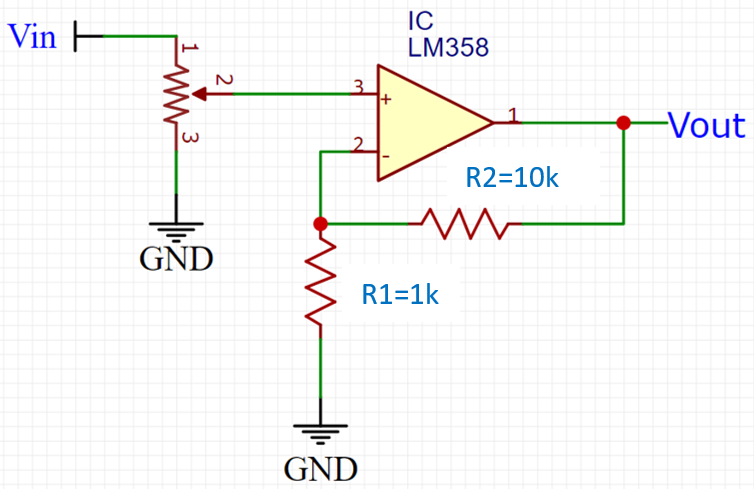
\includegraphics{EXP_09_Images/fig3.PNG}
\end{center}
\begin{center} {Figure 3.Expected step response without ripples}\end{center}

\noindent \textbf{\large PROCEDURE}\\[3pt]
This experiment is completed in two-step. In the first step, as shown in the circuit connection given below, we are supplying a square pulse to the RC circuit by using the Analog write function at pin number 6 of Arduino 1. The output of pin 6 is also connected to the Analog pin A0 and read through the Analog read function and the values are plotted/displayed in serial plotter/monitor. Here two Oscilloscopes are used (in Tinkercad only) one for showing supply signal and another for showing output signal across the capacitor. We don’t have an Oscilloscope thus, in actual hardware implementation the supply signal can be viewed in serial monitor instead of Oscilloscope (as we have read the output of pin 6 through Analog pin A0). The expected supply signal on the serial plotter is given in fig. 6. Now to visualize the output signal across the capacitor,  we have to follow step 2. 

\begin{center} 
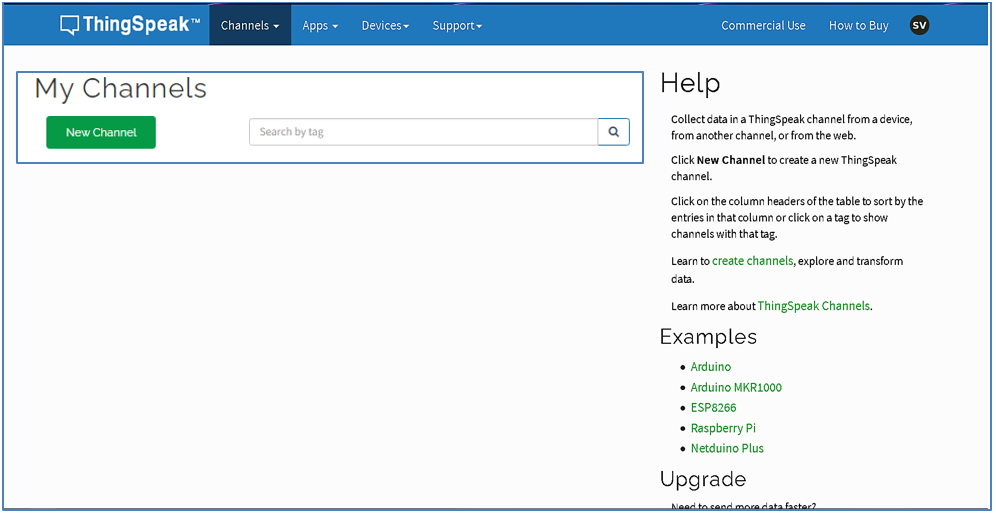
\includegraphics[scale=0.8]{EXP_09_Images/fig4.PNG}
\end{center}
\begin{center} {Figure 4. Square pulse supplied to RC circuit by  Arduino 1}\end{center}

\end{justify}


\hspace{2cm}\textbf{\large Code for Step 1:}\\[6pt]
\setlength{\parindent}{10eM}

  void setup() \\
  \{\\
 pinMode(6, OUTPUT);\\
  Serial.begin(9600);\\
\}\\[12pt]

void loop() \\
\{  \\                  
  analogWrite(6,255/2); \\
     \hspace{12pt}\textcolor{blue}{ // Change the value(255,255/3,255/4,255/5..) and see the result}\\
    float sqr=analogRead(A0)*5.0/1023;\\
    Serial.print(" ");\\
    Serial.println(sqr)\\
\}
\begin{justify}
\noindent In the \textbf{ second step}, we are going to use another Arduino 2 as an Oscilloscope to see the output signal across the capacitor. After flashing the code in  Arduino 1, we have to remove it from the PC and supply it through DC Adapter. Now connect Arduino 2 as given in the circuit diagram below. The positive terminal of the capacitor is connected to A0 of Arduino 2 and the negative terminal is connected to GND of Arduino 2. Arduino 2 is connected to the  PC and code is flashed on it. Now we can see the output signal on the serial plotter read by this Arduino 2. via A0. The expected plot on the serial monitor is shown in fig. 7. \end{justify}

\begin{center} 
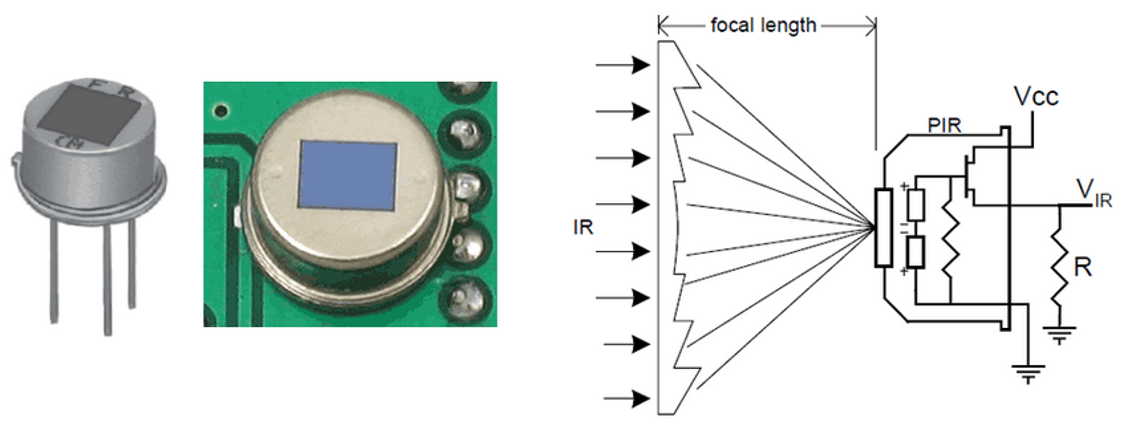
\includegraphics[scale=0.7]{EXP_09_Images/fig5.PNG}
\end{center}
\begin{center} {Figure 5.Output signal is being measured by Arduino 2}\end{center}

\hspace{2cm}\textbf{\large Code for Step 2:}\\[6pt]


\setlength{\parindent}{10eM}

  void setup() \\
  \{\\
  Serial.begin(9600);\\
\}\\[12pt]

void loop() \\
\{  \\                  
  float out=analogRead(A0)*5.0/1023;\\
    Serial.print(" ");\\
    Serial.println(out);\\

\}
\setlength{\parindent}{0pt}

\begin{justify}
\textbf{Expected Result:}\\
The following voltage waveforms are observed in the serial monitor. The first graph is the PWM signal generated by Arduino1. The second graph is the constant voltage across the capacitor measured by Arduino2.

\begin{center} 
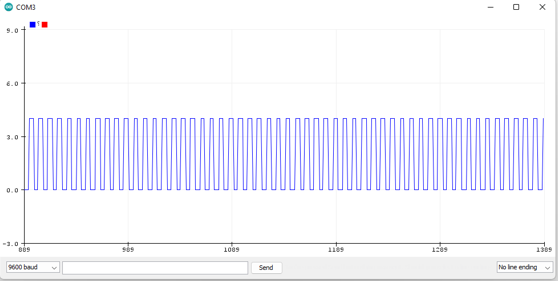
\includegraphics{EXP_09_Images/fig66.PNG}
\end{center}
\begin{center} {Figure 6.Supply signal to RC circuit}\end{center}

\begin{center} 
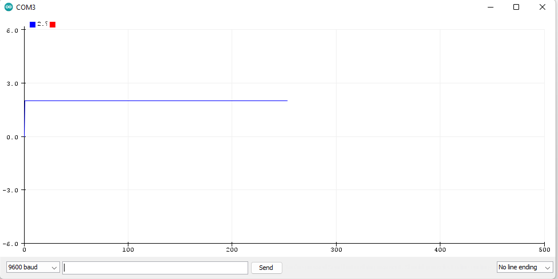
\includegraphics{EXP_09_Images/fig77.PNG}
\end{center}
\begin{center} {Figure 7.Output signal across the capacitor}\end{center}


\textbf{\large REFERENCES:}
\vspace{-6mm}
\begin{enumerate}
\setlength\itemsep{-0.3em}
\item  \href {https://www.arduino.cc/en/Reference/AnalogWrite}{AnalogWrite}
\item  \href {https://www.arduino.cc/en/Tutorial/SecretsOfArduinoPWM}{Arduino PWM}
\item  \href {https://developer.android.com/things/sdk/pio/pwm.html}{PWM}
\end{enumerate}

\end{justify}
\end{document}